\documentclass[border=4pt]{standalone}

% --- packages (mirror these in wandb.meta.json "requires") ---
\usepackage{tikz}
\usetikzlibrary{svg.path}

% --- brand color (Weights & Biases's official brand color; brand marks keep their
%     official color instead of the shared OpenTikZ palette by design) ---
\definecolor{brandwandb}{HTML}{FFBE00}

% Weights & Biases logo. Shape data derived from the CC0 simple-icons project
% (https://simple-icons.org), flattened to absolute M/L/C/Z commands with the
% y-axis pre-flipped for TikZ and scaled to ~2.5cm (svg.path ignores TikZ
% coordinate transforms, so the transform is baked into the coordinates).
% The Weights & Biases logo is a trademark of its owner; used here for identification.
\begin{document}
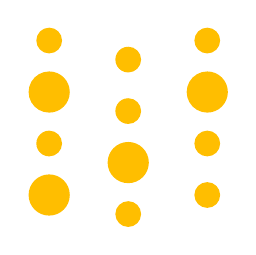
\begin{tikzpicture}
  \fill[brandwandb] svg {%
    M 7.44 72 C 4.8719 72 2.79 69.9181 2.79 67.35 C 2.79 64.7819 4.8719 62.7 7.44 62.7 C
    10.0081 62.7 12.09 64.7819 12.09 67.35 C 12.09 69.9181 10.0081 72 7.44 72 Z M 64.56
    72 C 61.991 72 59.9085 69.9175 59.9085 67.3485 C 59.9085 64.7795 61.991 62.697 64.56
    62.697 C 67.129 62.697 69.2115 64.7795 69.2115 67.3485 C 69.2115 69.9175 67.129 72
    64.56 72 Z M 36 65.115 C 34.3387 65.115 32.8036 64.2287 31.973 62.79 C 31.1423
    61.3513 31.1423 59.5787 31.973 58.14 C 32.8036 56.7013 34.3387 55.815 36 55.815 C
    38.5681 55.815 40.65 57.8969 40.65 60.465 C 40.65 63.0331 38.5681 65.115 36 65.115 Z
    M 7.44 56.184 C 4.7819 56.184 2.3258 54.7659 0.9968 52.464 C -0.3323 50.1621 -0.3323
    47.3259 0.9968 45.024 C 2.3258 42.7221 4.7819 41.304 7.44 41.304 C 11.549 41.304
    14.88 44.635 14.88 48.744 C 14.88 52.853 11.549 56.184 7.44 56.184 Z M 64.56 56.184
    C 61.9019 56.184 59.4458 54.7659 58.1168 52.464 C 56.7877 50.1621 56.7877 47.3259
    58.1168 45.024 C 59.4458 42.7221 61.9019 41.304 64.56 41.304 C 68.669 41.304 72
    44.635 72 48.744 C 72 52.853 68.669 56.184 64.56 56.184 Z M 36 46.512 C 34.3387
    46.512 32.8036 45.6257 31.973 44.187 C 31.1423 42.7483 31.1423 40.9757 31.973 39.537
    C 32.8036 38.0983 34.3387 37.212 36 37.212 C 38.5681 37.212 40.65 39.2939 40.65
    41.862 C 40.65 44.4301 38.5681 46.512 36 46.512 Z M 7.44 34.791 C 5.7787 34.791
    4.2436 33.9047 3.413 32.466 C 2.5823 31.0273 2.5823 29.2547 3.413 27.816 C 4.2436
    26.3773 5.7787 25.491 7.44 25.491 C 10.0081 25.491 12.09 27.5729 12.09 30.141 C
    12.09 32.7091 10.0081 34.791 7.44 34.791 Z M 64.56 34.791 C 61.9902 34.791 59.907
    32.7078 59.907 30.138 C 59.907 27.5682 61.9902 25.485 64.56 25.485 C 67.1298 25.485
    69.213 27.5682 69.213 30.138 C 69.213 32.7078 67.1298 34.791 64.56 34.791 Z M 36
    30.699 C 31.8893 30.699 28.557 27.3667 28.557 23.256 C 28.557 19.1453 31.8893 15.813
    36 15.813 C 40.1107 15.813 43.443 19.1453 43.443 23.256 C 43.443 27.3667 40.1107
    30.699 36 30.699 Z M 7.44 18.978 C 3.3293 18.9772 -0.0023 15.6442 -0.0015 11.5335 C
    -0.0007 7.4228 3.3323 4.0912 7.443 4.092 C 11.5537 4.092 14.886 7.4243 14.886 11.535
    C 14.886 15.6457 11.5537 18.978 7.443 18.978 Z M 64.56 16.188 C 61.9902 16.188
    59.907 14.1048 59.907 11.535 C 59.907 8.9652 61.9902 6.882 64.56 6.882 C 67.129
    6.882 69.2115 8.9645 69.2115 11.5335 C 69.2115 14.1025 67.129 16.185 64.56 16.185 Z
    M 36 9.3 C 33.4319 9.3 31.35 7.2181 31.35 4.65 C 31.35 2.0819 33.4319 0 36 0 C
    38.5681 0 40.65 2.0819 40.65 4.65 C 40.65 7.2181 38.5681 9.3 36 9.3 Z%
  };
\end{tikzpicture}
\end{document}
